%\documentclass{standalone}
%\usepackage{tikz}
%\usetikzlibrary{patterns,plotmarks}
%\begin{document}
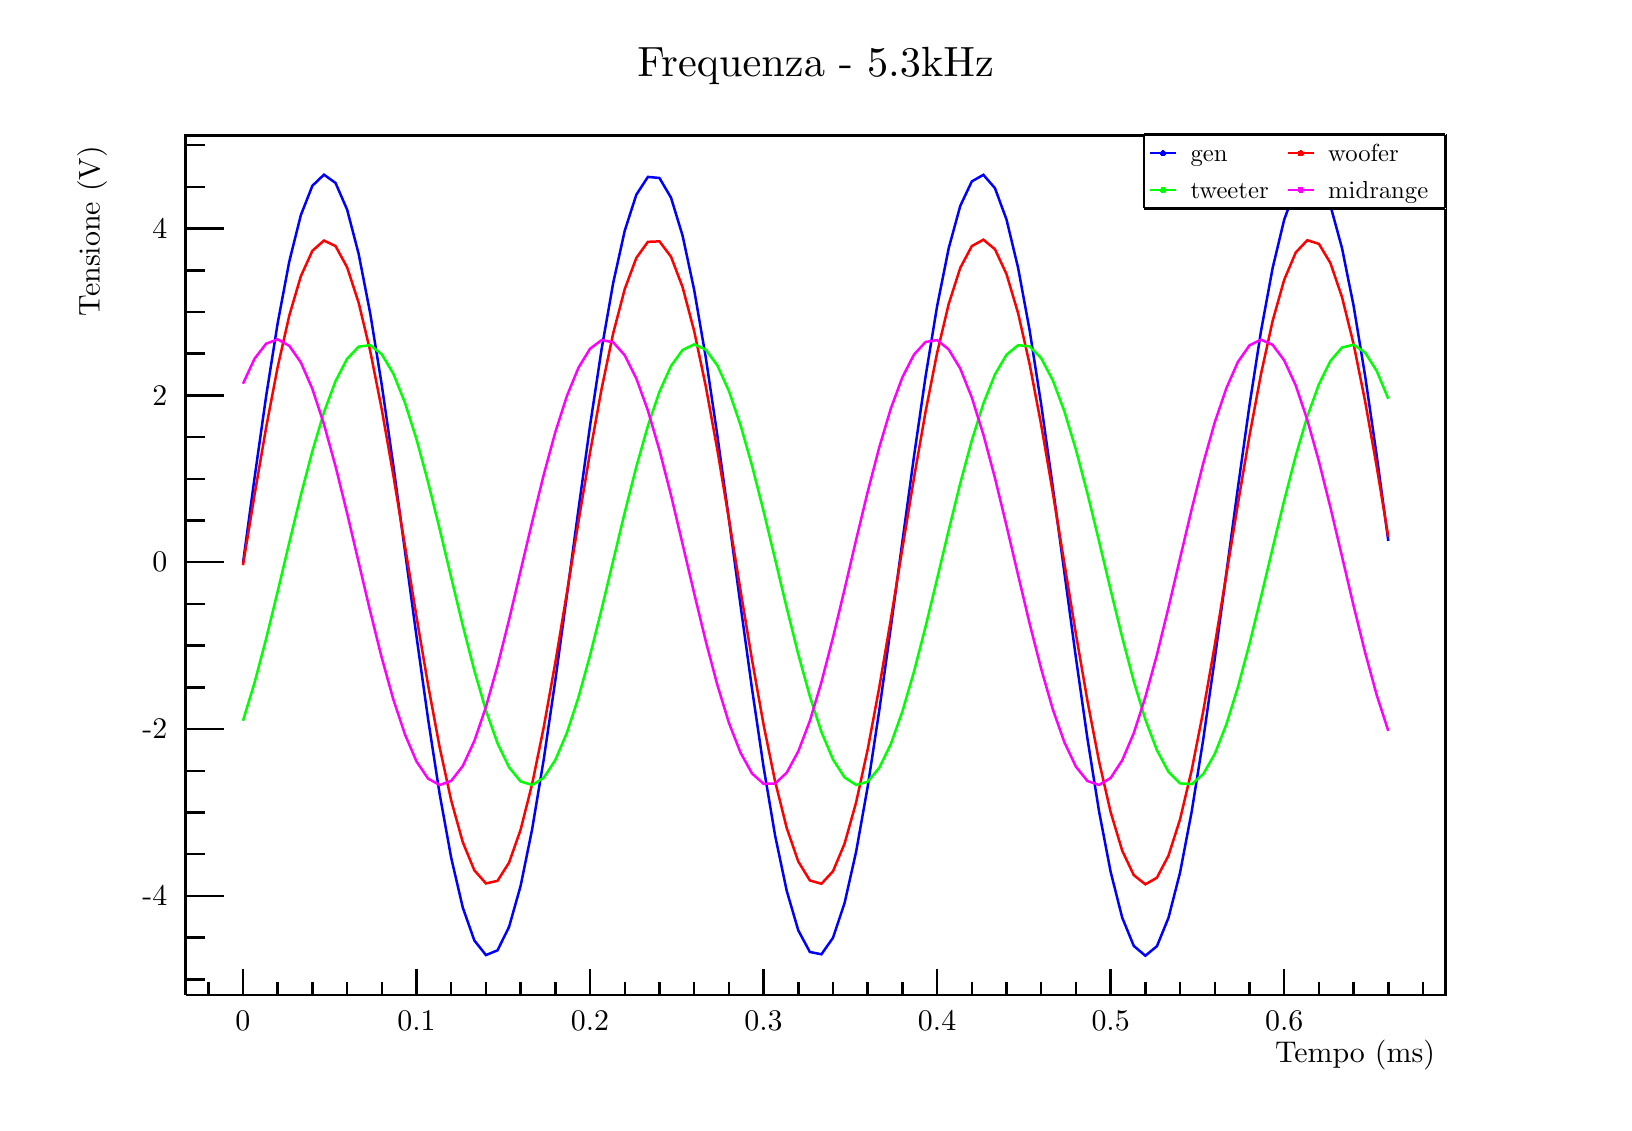
\begin{tikzpicture}
\def\CheckTikzLibraryLoaded#1{ \ifcsname tikz@library@#1@loaded\endcsname \else \PackageWarning{tikz}{usetikzlibrary{#1} is missing in the preamble.} \fi }
\CheckTikzLibraryLoaded{patterns}
\CheckTikzLibraryLoaded{plotmarks}
\pgfdeclareplotmark{cross} {
\pgfpathmoveto{\pgfpoint{-0.3\pgfplotmarksize}{\pgfplotmarksize}}
\pgfpathlineto{\pgfpoint{+0.3\pgfplotmarksize}{\pgfplotmarksize}}
\pgfpathlineto{\pgfpoint{+0.3\pgfplotmarksize}{0.3\pgfplotmarksize}}
\pgfpathlineto{\pgfpoint{+1\pgfplotmarksize}{0.3\pgfplotmarksize}}
\pgfpathlineto{\pgfpoint{+1\pgfplotmarksize}{-0.3\pgfplotmarksize}}
\pgfpathlineto{\pgfpoint{+0.3\pgfplotmarksize}{-0.3\pgfplotmarksize}}
\pgfpathlineto{\pgfpoint{+0.3\pgfplotmarksize}{-1.\pgfplotmarksize}}
\pgfpathlineto{\pgfpoint{-0.3\pgfplotmarksize}{-1.\pgfplotmarksize}}
\pgfpathlineto{\pgfpoint{-0.3\pgfplotmarksize}{-0.3\pgfplotmarksize}}
\pgfpathlineto{\pgfpoint{-1.\pgfplotmarksize}{-0.3\pgfplotmarksize}}
\pgfpathlineto{\pgfpoint{-1.\pgfplotmarksize}{0.3\pgfplotmarksize}}
\pgfpathlineto{\pgfpoint{-0.3\pgfplotmarksize}{0.3\pgfplotmarksize}}
\pgfpathclose
\pgfusepathqstroke
}
\pgfdeclareplotmark{cross*} {
\pgfpathmoveto{\pgfpoint{-0.3\pgfplotmarksize}{\pgfplotmarksize}}
\pgfpathlineto{\pgfpoint{+0.3\pgfplotmarksize}{\pgfplotmarksize}}
\pgfpathlineto{\pgfpoint{+0.3\pgfplotmarksize}{0.3\pgfplotmarksize}}
\pgfpathlineto{\pgfpoint{+1\pgfplotmarksize}{0.3\pgfplotmarksize}}
\pgfpathlineto{\pgfpoint{+1\pgfplotmarksize}{-0.3\pgfplotmarksize}}
\pgfpathlineto{\pgfpoint{+0.3\pgfplotmarksize}{-0.3\pgfplotmarksize}}
\pgfpathlineto{\pgfpoint{+0.3\pgfplotmarksize}{-1.\pgfplotmarksize}}
\pgfpathlineto{\pgfpoint{-0.3\pgfplotmarksize}{-1.\pgfplotmarksize}}
\pgfpathlineto{\pgfpoint{-0.3\pgfplotmarksize}{-0.3\pgfplotmarksize}}
\pgfpathlineto{\pgfpoint{-1.\pgfplotmarksize}{-0.3\pgfplotmarksize}}
\pgfpathlineto{\pgfpoint{-1.\pgfplotmarksize}{0.3\pgfplotmarksize}}
\pgfpathlineto{\pgfpoint{-0.3\pgfplotmarksize}{0.3\pgfplotmarksize}}
\pgfpathclose
\pgfusepathqfillstroke
}
\pgfdeclareplotmark{newstar} {
\pgfpathmoveto{\pgfqpoint{0pt}{\pgfplotmarksize}}
\pgfpathlineto{\pgfqpointpolar{44}{0.5\pgfplotmarksize}}
\pgfpathlineto{\pgfqpointpolar{18}{\pgfplotmarksize}}
\pgfpathlineto{\pgfqpointpolar{-20}{0.5\pgfplotmarksize}}
\pgfpathlineto{\pgfqpointpolar{-54}{\pgfplotmarksize}}
\pgfpathlineto{\pgfqpointpolar{-90}{0.5\pgfplotmarksize}}
\pgfpathlineto{\pgfqpointpolar{234}{\pgfplotmarksize}}
\pgfpathlineto{\pgfqpointpolar{198}{0.5\pgfplotmarksize}}
\pgfpathlineto{\pgfqpointpolar{162}{\pgfplotmarksize}}
\pgfpathlineto{\pgfqpointpolar{134}{0.5\pgfplotmarksize}}
\pgfpathclose
\pgfusepathqstroke
}
\pgfdeclareplotmark{newstar*} {
\pgfpathmoveto{\pgfqpoint{0pt}{\pgfplotmarksize}}
\pgfpathlineto{\pgfqpointpolar{44}{0.5\pgfplotmarksize}}
\pgfpathlineto{\pgfqpointpolar{18}{\pgfplotmarksize}}
\pgfpathlineto{\pgfqpointpolar{-20}{0.5\pgfplotmarksize}}
\pgfpathlineto{\pgfqpointpolar{-54}{\pgfplotmarksize}}
\pgfpathlineto{\pgfqpointpolar{-90}{0.5\pgfplotmarksize}}
\pgfpathlineto{\pgfqpointpolar{234}{\pgfplotmarksize}}
\pgfpathlineto{\pgfqpointpolar{198}{0.5\pgfplotmarksize}}
\pgfpathlineto{\pgfqpointpolar{162}{\pgfplotmarksize}}
\pgfpathlineto{\pgfqpointpolar{134}{0.5\pgfplotmarksize}}
\pgfpathclose
\pgfusepathqfillstroke
}
\definecolor{c}{rgb}{1,1,1};
\draw [color=c, fill=c] (0,0) rectangle (20,13.639);
\draw [color=c, fill=c] (2,1.3639) rectangle (18,12.2751);
\definecolor{c}{rgb}{0,0,0};
\draw [c,line width=0.9] (2,1.3639) -- (2,12.2751) -- (18,12.2751) -- (18,1.3639) -- (2,1.3639);
\definecolor{c}{rgb}{1,1,1};
\draw [color=c, fill=c] (2,1.3639) rectangle (18,12.2751);
\definecolor{c}{rgb}{0,0,0};
\draw [c,line width=0.9] (2,1.3639) -- (2,12.2751) -- (18,12.2751) -- (18,1.3639) -- (2,1.3639);
\draw [c,line width=0.9] (2,1.3639) -- (18,1.3639);
\draw [c,line width=0.9] (2.72727,1.69123) -- (2.72727,1.3639);
\draw [c,line width=0.9] (3.16804,1.52756) -- (3.16804,1.3639);
\draw [c,line width=0.9] (3.60882,1.52756) -- (3.60882,1.3639);
\draw [c,line width=0.9] (4.04959,1.52756) -- (4.04959,1.3639);
\draw [c,line width=0.9] (4.49036,1.52756) -- (4.49036,1.3639);
\draw [c,line width=0.9] (4.93113,1.69123) -- (4.93113,1.3639);
\draw [c,line width=0.9] (5.3719,1.52756) -- (5.3719,1.3639);
\draw [c,line width=0.9] (5.81267,1.52756) -- (5.81267,1.3639);
\draw [c,line width=0.9] (6.25344,1.52756) -- (6.25344,1.3639);
\draw [c,line width=0.9] (6.69421,1.52756) -- (6.69421,1.3639);
\draw [c,line width=0.9] (7.13499,1.69123) -- (7.13499,1.3639);
\draw [c,line width=0.9] (7.57576,1.52756) -- (7.57576,1.3639);
\draw [c,line width=0.9] (8.01653,1.52756) -- (8.01653,1.3639);
\draw [c,line width=0.9] (8.4573,1.52756) -- (8.4573,1.3639);
\draw [c,line width=0.9] (8.89807,1.52756) -- (8.89807,1.3639);
\draw [c,line width=0.9] (9.33884,1.69123) -- (9.33884,1.3639);
\draw [c,line width=0.9] (9.77961,1.52756) -- (9.77961,1.3639);
\draw [c,line width=0.9] (10.2204,1.52756) -- (10.2204,1.3639);
\draw [c,line width=0.9] (10.6612,1.52756) -- (10.6612,1.3639);
\draw [c,line width=0.9] (11.1019,1.52756) -- (11.1019,1.3639);
\draw [c,line width=0.9] (11.5427,1.69123) -- (11.5427,1.3639);
\draw [c,line width=0.9] (11.9835,1.52756) -- (11.9835,1.3639);
\draw [c,line width=0.9] (12.4242,1.52756) -- (12.4242,1.3639);
\draw [c,line width=0.9] (12.865,1.52756) -- (12.865,1.3639);
\draw [c,line width=0.9] (13.3058,1.52756) -- (13.3058,1.3639);
\draw [c,line width=0.9] (13.7466,1.69123) -- (13.7466,1.3639);
\draw [c,line width=0.9] (14.1873,1.52756) -- (14.1873,1.3639);
\draw [c,line width=0.9] (14.6281,1.52756) -- (14.6281,1.3639);
\draw [c,line width=0.9] (15.0689,1.52756) -- (15.0689,1.3639);
\draw [c,line width=0.9] (15.5096,1.52756) -- (15.5096,1.3639);
\draw [c,line width=0.9] (15.9504,1.69123) -- (15.9504,1.3639);
\draw [c,line width=0.9] (2.72727,1.69123) -- (2.72727,1.3639);
\draw [c,line width=0.9] (2.2865,1.52756) -- (2.2865,1.3639);
\draw [c,line width=0.9] (15.9504,1.69123) -- (15.9504,1.3639);
\draw [c,line width=0.9] (16.3912,1.52756) -- (16.3912,1.3639);
\draw [c,line width=0.9] (16.832,1.52756) -- (16.832,1.3639);
\draw [c,line width=0.9] (17.2727,1.52756) -- (17.2727,1.3639);
\draw [c,line width=0.9] (17.7135,1.52756) -- (17.7135,1.3639);
\draw [anchor=base] (2.72727,0.913811) node[scale=1.08185, color=c, rotate=0]{0};
\draw [anchor=base] (4.93113,0.913811) node[scale=1.08185, color=c, rotate=0]{0.1};
\draw [anchor=base] (7.13499,0.913811) node[scale=1.08185, color=c, rotate=0]{0.2};
\draw [anchor=base] (9.33884,0.913811) node[scale=1.08185, color=c, rotate=0]{0.3};
\draw [anchor=base] (11.5427,0.913811) node[scale=1.08185, color=c, rotate=0]{0.4};
\draw [anchor=base] (13.7466,0.913811) node[scale=1.08185, color=c, rotate=0]{0.5};
\draw [anchor=base] (15.9504,0.913811) node[scale=1.08185, color=c, rotate=0]{0.6};
\draw [anchor= east] (18,0.600115) node[scale=1.08185, color=c, rotate=0]{ Tempo (ms)};
\draw [c,line width=0.9] (2,1.3639) -- (2,12.2751);
\draw [c,line width=0.9] (2.48,2.61904) -- (2,2.61904);
\draw [c,line width=0.9] (2.24,3.14877) -- (2,3.14877);
\draw [c,line width=0.9] (2.24,3.6785) -- (2,3.6785);
\draw [c,line width=0.9] (2.24,4.20823) -- (2,4.20823);
\draw [c,line width=0.9] (2.48,4.73797) -- (2,4.73797);
\draw [c,line width=0.9] (2.24,5.2677) -- (2,5.2677);
\draw [c,line width=0.9] (2.24,5.79743) -- (2,5.79743);
\draw [c,line width=0.9] (2.24,6.32717) -- (2,6.32717);
\draw [c,line width=0.9] (2.48,6.8569) -- (2,6.8569);
\draw [c,line width=0.9] (2.24,7.38663) -- (2,7.38663);
\draw [c,line width=0.9] (2.24,7.91637) -- (2,7.91637);
\draw [c,line width=0.9] (2.24,8.4461) -- (2,8.4461);
\draw [c,line width=0.9] (2.48,8.97583) -- (2,8.97583);
\draw [c,line width=0.9] (2.24,9.50557) -- (2,9.50557);
\draw [c,line width=0.9] (2.24,10.0353) -- (2,10.0353);
\draw [c,line width=0.9] (2.24,10.565) -- (2,10.565);
\draw [c,line width=0.9] (2.48,11.0948) -- (2,11.0948);
\draw [c,line width=0.9] (2.48,2.61904) -- (2,2.61904);
\draw [c,line width=0.9] (2.24,2.0893) -- (2,2.0893);
\draw [c,line width=0.9] (2.24,1.55957) -- (2,1.55957);
\draw [c,line width=0.9] (2.48,11.0948) -- (2,11.0948);
\draw [c,line width=0.9] (2.24,11.6245) -- (2,11.6245);
\draw [c,line width=0.9] (2.24,12.1542) -- (2,12.1542);
\draw [anchor= east] (1.9,2.61904) node[scale=1.08185, color=c, rotate=0]{-4};
\draw [anchor= east] (1.9,4.73797) node[scale=1.08185, color=c, rotate=0]{-2};
\draw [anchor= east] (1.9,6.8569) node[scale=1.08185, color=c, rotate=0]{0};
\draw [anchor= east] (1.9,8.97583) node[scale=1.08185, color=c, rotate=0]{2};
\draw [anchor= east] (1.9,11.0948) node[scale=1.08185, color=c, rotate=0]{4};
\draw [anchor= east] (0.812894,12.2751) node[scale=1.08185, color=c, rotate=90]{ Tensione (V)};
\definecolor{c}{rgb}{0,0,1};
\draw [c,line width=0.9] (2.72727,6.84364) -- (2.8742,7.92827) -- (3.02112,8.96413) -- (3.16804,9.89408) -- (3.31497,10.6746) -- (3.46189,11.2643) -- (3.60882,11.6382) -- (3.75574,11.7791) -- (3.90266,11.674) -- (4.04959,11.3363) -- (4.19651,10.772)
 -- (4.34343,10.0162) -- (4.49036,9.1057) -- (4.63728,8.08417) -- (4.78421,7.00022) -- (4.93113,5.91424) -- (5.07805,4.8656) -- (5.22498,3.913) -- (5.3719,3.10212) -- (5.51882,2.47135) -- (5.66575,2.05329) -- (5.81267,1.86822) -- (5.9596,1.92775) --
 (6.10652,2.22608) -- (6.25344,2.74682) -- (6.40037,3.47055) -- (6.54729,4.3551) -- (6.69421,5.35888) -- (6.84114,6.43804) -- (6.98806,7.52846) -- (7.13499,8.59093) -- (7.28191,9.56454) -- (7.42883,10.4026) -- (7.57576,11.0678) -- (7.72268,11.5243)
 -- (7.86961,11.7506) -- (8.01653,11.737) -- (8.16345,11.4867) -- (8.31038,11.0043) -- (8.4573,10.3162) -- (8.60422,9.46151) -- (8.75115,8.47221) -- (8.89807,7.40839) -- (9.045,6.31779) -- (9.19192,5.25074) -- (9.33884,4.25566) -- (9.48577,3.38356)
 -- (9.63269,2.6844) -- (9.77961,2.18173) -- (9.92654,1.90745) -- (10.0735,1.87794) -- (10.2204,2.0874) -- (10.3673,2.52816) -- (10.5142,3.18075) -- (10.6612,4.00681) -- (10.8081,4.97511) -- (10.955,6.03176) -- (11.1019,7.12235) -- (11.2489,8.20016)
 -- (11.3958,9.21401) -- (11.5427,10.1093) -- (11.6896,10.8438) -- (11.8365,11.3818) -- (11.9835,11.6935) -- (12.1304,11.7771) -- (12.2773,11.6078) -- (12.4242,11.2085) -- (12.5712,10.5965) -- (12.7181,9.80026) -- (12.865,8.85684) -- (13.0119,7.8128)
 -- (13.1589,6.72613) -- (13.3058,5.6415) -- (13.4527,4.61095) -- (13.5996,3.69177) -- (13.7466,2.92473) -- (13.8935,2.3436) -- (14.0404,1.98438) -- (14.1873,1.85986) -- (14.3343,1.98079) -- (14.4812,2.34121) -- (14.6281,2.91654) -- (14.775,3.68546)
 -- (14.9219,4.60259) -- (15.0689,5.63042) -- (15.2158,6.71674) -- (15.3627,7.80291) -- (15.5096,8.849) -- (15.6566,9.79498) -- (15.8035,10.5921) -- (15.9504,11.2072) -- (16.0973,11.6084) -- (16.2443,11.7706) -- (16.3912,11.6964) -- (16.5381,11.3851)
 -- (16.685,10.8454) -- (16.832,10.1139) -- (16.9789,9.22066) -- (17.1258,8.20937) -- (17.2727,7.12798);
\definecolor{c}{rgb}{1,0,0};
\draw [c,line width=0.9] (2.72727,6.81942) -- (2.8742,7.71302) -- (3.02112,8.56636) -- (3.16804,9.33751) -- (3.31497,9.9884) -- (3.46189,10.4885) -- (3.60882,10.8123) -- (3.75574,10.9424) -- (3.90266,10.8721) -- (4.04959,10.6037) -- (4.19651,10.1518)
 -- (4.34343,9.53827) -- (4.49036,8.79458) -- (4.63728,7.95727) -- (4.78421,7.06623) -- (4.93113,6.16531) -- (5.07805,5.29799) -- (5.22498,4.50742) -- (5.3719,3.83078) -- (5.51882,3.30134) -- (5.66575,2.94417) -- (5.81267,2.77787) -- (5.9596,2.81079)
 -- (6.10652,3.04208) -- (6.25344,3.46082) -- (6.40037,4.04382) -- (6.54729,4.76378) -- (6.69421,5.58488) -- (6.84114,6.46908) -- (6.98806,7.37189) -- (7.13499,8.25013) -- (7.28191,9.06033) -- (7.42883,9.7641) -- (7.57576,10.3265) --
 (7.72268,10.7214) -- (7.86961,10.9262) -- (8.01653,10.932) -- (8.16345,10.7364) -- (8.31038,10.35) -- (8.4573,9.79327) -- (8.60422,9.09376) -- (8.75115,8.28595) -- (8.89807,7.40839) -- (9.045,6.5049) -- (9.19192,5.61848) -- (9.33884,4.79346) --
 (9.48577,4.06992) -- (9.63269,3.48197) -- (9.77961,3.05624) -- (9.92654,2.81591) -- (10.0735,2.7736) -- (10.2204,2.93223) -- (10.3673,3.28275) -- (10.5142,3.80758) -- (10.6612,4.4803) -- (10.8081,5.26831) -- (10.955,6.13324) -- (11.1019,7.03348) --
 (11.2489,7.92674) -- (11.3958,8.76797) -- (11.5427,9.51592) -- (11.6896,10.1353) -- (11.8365,10.5948) -- (11.9835,10.8721) -- (12.1304,10.9532) -- (12.2773,10.8321) -- (12.4242,10.5158) -- (12.5712,10.02) -- (12.7181,9.36991) -- (12.865,8.59758) --
 (13.0119,7.74116) -- (13.1589,6.84211) -- (13.3058,5.94443) -- (13.4527,5.09211) -- (13.5996,4.32611) -- (13.7466,3.68307) -- (13.8935,3.19371) -- (14.0404,2.88345) -- (14.1873,2.76661) -- (14.3343,2.85087) -- (14.4812,3.13129) -- (14.6281,3.59284)
 -- (14.775,4.2137) -- (14.9219,4.96283) -- (15.0689,5.80439) -- (15.2158,6.69679) -- (15.3627,7.59789) -- (15.5096,8.46283) -- (15.6566,9.24983) -- (15.8035,9.92086) -- (15.9504,10.4432) -- (16.0973,10.7908) -- (16.2443,10.9467) -- (16.3912,10.9003)
 -- (16.5381,10.6553) -- (16.685,10.2233) -- (16.832,9.62765) -- (16.9789,8.89744) -- (17.1258,8.06831) -- (17.2727,7.18);
\definecolor{c}{rgb}{0,1,0};
\draw [c,line width=0.9] (2.72727,4.8436) -- (2.8742,5.32698) -- (3.02112,5.88473) -- (3.16804,6.48716) -- (3.31497,7.10512) -- (3.46189,7.70909) -- (3.60882,8.26958) -- (3.75574,8.76098) -- (3.90266,9.15738) -- (4.04959,9.43968) -- (4.19651,9.59455)
 -- (4.34343,9.61434) -- (4.49036,9.49733) -- (4.63728,9.25) -- (4.78421,8.88345) -- (4.93113,8.41746) -- (5.07805,7.87369) -- (5.22498,7.27859) -- (5.3719,6.66165) -- (5.51882,6.05222) -- (5.66575,5.481) -- (5.81267,4.9746) -- (5.9596,4.55859) --
 (6.10652,4.25293) -- (6.25344,4.07282) -- (6.40037,4.02813) -- (6.54729,4.1204) -- (6.69421,4.34521) -- (6.84114,4.6918) -- (6.98806,5.14209) -- (7.13499,5.67408) -- (7.28191,6.26168) -- (7.42883,6.87725) -- (7.57576,7.49009) -- (7.72268,8.06967) --
 (7.86961,8.58939) -- (8.01653,9.02246) -- (8.16345,9.34962) -- (8.31038,9.55242) -- (8.4573,9.62372) -- (8.60422,9.55737) -- (8.75115,9.3578) -- (8.89807,9.03236) -- (9.045,8.60116) -- (9.19192,8.08332) -- (9.33884,7.50424) -- (9.48577,6.89208) --
 (9.63269,6.27703) -- (9.77961,5.68773) -- (9.92654,5.15403) -- (10.0735,4.70135) -- (10.2204,4.3522) -- (10.3673,4.1245) -- (10.5142,4.02847) -- (10.6612,4.06957) -- (10.8081,4.24628) -- (10.955,4.54869) -- (11.1019,4.96266) -- (11.2489,5.46736) --
 (11.3958,6.03824) -- (11.5427,6.64715) -- (11.6896,7.26426) -- (11.8365,7.85919) -- (11.9835,8.40501) -- (12.1304,8.87288) -- (12.2773,9.24165) -- (12.4242,9.49238) -- (12.5712,9.61349) -- (12.7181,9.59831) -- (12.865,9.44735) -- (13.0119,9.16762)
 -- (13.1589,8.77343) -- (13.3058,8.2851) -- (13.4527,7.72598) -- (13.5996,7.12167) -- (13.7466,6.50422) -- (13.8935,5.90196) -- (14.0404,5.34472) -- (14.1873,4.85912) -- (14.3343,4.46955) -- (14.4812,4.1946) -- (14.6281,4.04842) -- (14.775,4.03819)
 -- (14.9219,4.16492) -- (15.0689,4.42231) -- (15.2158,4.79721) -- (15.3627,5.2707) -- (15.5096,5.81991) -- (15.6566,6.41774) -- (15.8035,7.03519) -- (15.9504,7.64155) -- (16.0973,8.20902) -- (16.2443,8.7093) -- (16.3912,9.11679) -- (16.5381,9.41358)
 -- (16.685,9.58398) -- (16.832,9.6198) -- (16.9789,9.51882) -- (17.1258,9.28599) -- (17.2727,8.93291);
\definecolor{c}{rgb}{1,0,1};
\draw [c,line width=0.9] (2.72727,9.12412) -- (2.8742,9.44172) -- (3.02112,9.63276) -- (3.16804,9.68786) -- (3.31497,9.60564) -- (3.46189,9.3955) -- (3.60882,9.05743) -- (3.75574,8.60952) -- (3.90266,8.07513) -- (4.04959,7.48071) -- (4.19651,6.85439)
 -- (4.34343,6.23115) -- (4.49036,5.64185) -- (4.63728,5.11224) -- (4.78421,4.67099) -- (4.93113,4.32696) -- (5.07805,4.10915) -- (5.22498,4.02727) -- (5.3719,4.08049) -- (5.51882,4.26931) -- (5.66575,4.58741) -- (5.81267,5.01809) -- (5.9596,5.54036)
 -- (6.10652,6.12557) -- (6.25344,6.75052) -- (6.40037,7.37086) -- (6.54729,7.96938) -- (6.69421,8.51008) -- (6.84114,8.96805) -- (6.98806,9.32727) -- (7.13499,9.56846) -- (7.28191,9.67865) -- (7.42883,9.65016) -- (7.57576,9.48488) --
 (7.72268,9.19082) -- (7.86961,8.78401) -- (8.01653,8.28015) -- (8.16345,7.70722) -- (8.31038,7.08602) -- (8.4573,6.46226) -- (8.60422,5.8559) -- (8.75115,5.30071) -- (8.89807,4.81887) -- (9.045,4.4409) -- (9.19192,4.17447) -- (9.33884,4.0428) --
 (9.48577,4.04655) -- (9.63269,4.18437) -- (9.77961,4.45522) -- (9.92654,4.84156) -- (10.0735,5.33398) -- (10.2204,5.90008) -- (10.3673,6.51326) -- (10.5142,7.1423) -- (10.6612,7.75174) -- (10.8081,8.31614) -- (10.955,8.80942) -- (11.1019,9.20531) --
 (11.2489,9.49392) -- (11.3958,9.65408) -- (11.5427,9.67865) -- (11.6896,9.55993) -- (11.8365,9.3167) -- (11.9835,8.9481) -- (12.1304,8.47682) -- (12.2773,7.92657) -- (12.4242,7.31986) -- (12.5712,6.69372) -- (12.7181,6.07576) -- (12.865,5.50096) --
 (13.0119,4.98892) -- (13.1589,4.57138) -- (13.3058,4.25976) -- (13.4527,4.07759) -- (13.5996,4.02847) -- (13.7466,4.11716) -- (13.8935,4.34112) -- (14.0404,4.68668) -- (14.1873,5.14431) -- (14.3343,5.68176) -- (14.4812,6.28146) -- (14.6281,6.90761)
 -- (14.775,7.52744) -- (14.9219,8.11146) -- (15.0689,8.63391) -- (15.2158,9.06613) -- (15.3627,9.40045) -- (15.5096,9.61093) -- (15.6566,9.6841) -- (15.8035,9.61843) -- (15.9504,9.42109) -- (16.0973,9.10178) -- (16.2443,8.6641) -- (16.3912,8.13909)
 -- (16.5381,7.55047) -- (16.685,6.9291) -- (16.832,6.30364) -- (16.9789,5.70871) -- (17.1258,5.16921) -- (17.2727,4.715);
\definecolor{c}{rgb}{1,1,1};
\draw [color=c, fill=c] (14.1728,11.3519) rectangle (17.9941,12.2868);
\definecolor{c}{rgb}{0,0,0};
\draw [c,line width=0.9] (14.1728,11.3519) -- (17.9941,11.3519);
\draw [c,line width=0.9] (17.9941,11.3519) -- (17.9941,12.2868);
\draw [c,line width=0.9] (17.9941,12.2868) -- (14.1728,12.2868);
\draw [c,line width=0.9] (14.1728,12.2868) -- (14.1728,11.3519);
\draw [anchor=base west] (14.6504,11.9479) node[scale=0.890934, color=c, rotate=0]{gen};
\definecolor{c}{rgb}{1,1,1};
\draw [c, fill=c] (14.2444,11.8894) -- (14.5788,11.8894) -- (14.5788,12.2166) -- (14.2444,12.2166);
\definecolor{c}{rgb}{0,0,1};
\draw [c,line width=0.9] (14.2444,12.053) -- (14.5788,12.053);
\foreach \P in {(14.4116,12.053)}{\draw[mark options={color=c,fill=c},mark size=2.402402pt, line width=0.000000pt, mark=*,mark size=1pt] plot coordinates {\P};}
\definecolor{c}{rgb}{0,0,0};
\draw [anchor=base west] (16.3986,11.9479) node[scale=0.890934, color=c, rotate=0]{woofer};
\definecolor{c}{rgb}{1,1,1};
\draw [c, fill=c] (15.9926,11.8894) -- (16.327,11.8894) -- (16.327,12.2166) -- (15.9926,12.2166);
\definecolor{c}{rgb}{1,0,0};
\draw [c,line width=0.9] (15.9926,12.053) -- (16.327,12.053);
\foreach \P in {(16.1598,12.053)}{\draw[mark options={color=c,fill=c},mark size=2.402402pt, line width=0.000000pt, mark=*,mark size=1pt] plot coordinates {\P};}
\definecolor{c}{rgb}{0,0,0};
\draw [anchor=base west] (14.6504,11.4804) node[scale=0.890934, color=c, rotate=0]{tweeter};
\definecolor{c}{rgb}{1,1,1};
\draw [c, fill=c] (14.2444,11.422) -- (14.5788,11.422) -- (14.5788,11.7492) -- (14.2444,11.7492);
\definecolor{c}{rgb}{0,1,0};
\draw [c,line width=0.9] (14.2444,11.5856) -- (14.5788,11.5856);
\foreach \P in {(14.4116,11.5856)}{\draw[mark options={color=c,fill=c},mark size=2.402402pt, line width=0.000000pt, mark=*,mark size=1pt] plot coordinates {\P};}
\definecolor{c}{rgb}{0,0,0};
\draw [anchor=base west] (16.3986,11.4804) node[scale=0.890934, color=c, rotate=0]{midrange};
\definecolor{c}{rgb}{1,1,1};
\draw [c, fill=c] (15.9926,11.422) -- (16.327,11.422) -- (16.327,11.7492) -- (15.9926,11.7492);
\definecolor{c}{rgb}{1,0,1};
\draw [c,line width=0.9] (15.9926,11.5856) -- (16.327,11.5856);
\foreach \P in {(16.1598,11.5856)}{\draw[mark options={color=c,fill=c},mark size=2.402402pt, line width=0.000000pt, mark=*,mark size=1pt] plot coordinates {\P};}
\definecolor{c}{rgb}{0,0,0};
\draw (10,13.1582) node[scale=1.52731, color=c, rotate=0]{Frequenza - 5.3kHz};
\end{tikzpicture}
%\end{document}
